\setchaptergraphic{
    % Hyperboloid of one sheet
    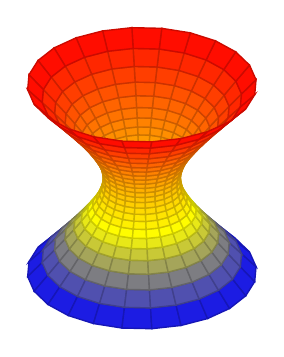
\begin{tikzpicture}[scale=1.25]
        \begin{axis}[hide axis,axis equal,colormap/hot]
            \addplot3[surf,domain=0:360,y domain=-1.75:1.75] ({cosh(y)*cos(x)},{cosh(y)*sin(x)},{sinh(y)});
        \end{axis}
    \end{tikzpicture}
    \hspace{1cm}
    % Saddle
    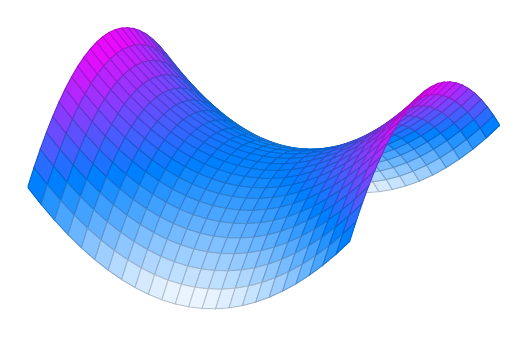
\begin{tikzpicture}[scale=0.875]
        \begin{axis}[hide axis,colormap/cool]
            \addplot3[surf,domain=-1.5:1.5,y domain=-1.5:1.5] {x^2-y^2};
        \end{axis}
    \end{tikzpicture}
}

\chapter{Vector Calculus}
\label{ch:vector-calc}

\section{Orthogonal Projection}

\begin{thm}\label{law-of-cosines}
    Let $\theta$ be the angle between non-zero vectors $A$ and $B$, and let $C = A - B$. The \emph{Law of Cosines} states that $\norm{C}^2 = \norm{A}^2 + \norm{B}^2 - 2\norm{A}\norm{B}\cos(\theta)$.
\end{thm}

\begin{figure}[ht!]
    \centering
    \begin{tikzpicture}[scale=1.4]
        \coordinate (O) at (0, 0);
        \coordinate (A) at (3, 5);
        \coordinate (B) at (6, 2);
        \coordinate (A') at ($(O)!(A)!(B)$);

        \draw [thick, ->] (O) -- (A);
        \draw [thick, ->] (O) -- (B);
        \draw [thick, dashed] (A') -- (A);
        \draw [very thick, red, ->] (O) -- (A');

        \draw [decorate,decoration={brace,amplitude=6pt,raise=3pt]}]
            (O) -- (A) node [black,midway,xshift=-0.6cm,yshift=0.3cm]
            {\footnotesize $A$};

        \draw [decorate,decoration={brace,amplitude=6pt,raise=3pt]}]
            (B) -- (O) node [black,midway,xshift=0.2cm,yshift=-0.5cm]
            {\footnotesize $B$};

        \draw [decorate,decoration={brace,amplitude=6pt,raise=3pt]}]
            (A) -- (A') node [black,midway,xshift=1.0cm, yshift=0.1cm]
            {\footnotesize $A - A'$};

        \draw [decorate,decoration={brace,amplitude=6pt,raise=3pt]}]
            (O) -- (A') node [black,midway,xshift=-0.2cm, yshift=0.5cm]
            {\footnotesize $A'$};

        \tkzMarkAngle[size=1cm,mark=|](B,O,A)
        \tkzLabelAngle[pos=1.2](B,O,A) {$\theta$}

        \tkzMarkRightAngle[size=0.4](A,A',O)
    \end{tikzpicture}
\caption{Orthogonal projection of $\vec{A}$ onto $\vec{B}$}
\label{fig:orthogonal-projection}
\end{figure}

Figure \ref{fig:orthogonal-projection} shows $A'$, the orthogonal projection of vector $A$ onto $B$. $\norm{A'}$ is the shortest distance between the head of $A$ and $B$.

\begin{thm}
    Let $\theta$ be the angle between non-zero vectors $A$ and $B$. Then $\cos\theta = \frac{A \cdot B}{\norm{A}\norm{B}}$.
\end{thm}

\begin{proof}\label{vector-angle}
    Let $C = A - B$. Then $C \cdot C = (A - B) \cdot (A - B)$, which can we expand to get $A \cdot (A - B) - B \cdot (A - B) = A \cdot A + B \cdot B - 2(A \cdot B)$. Therefore, $\norm{C}^2 = \norm{A}^2 + \norm{B}^2 - 2(A \cdot B)$. By the Law of Cosines \ref{law-of-cosines} and transitivity, it follows that $A \cdot B = \norm{A}\norm{B}\cos\theta$, so $\cos\theta = \frac{A \cdot B}{\norm{A}\norm{B}}$.
\end{proof}

\begin{exmp}
    Let $A = \left(0, 1\right)$, and $B = \left(2, 2\right)$. Then $\cos\theta = \frac{A \cdot B}{\norm{A}\norm{B}}$. Since $A \cdot B = 0 \cdot 2 + 1 \cdot 2 = 2$, $\norm{A} = \sqrt{0^2 + 1^2} = 1$, and $\norm{B} = \sqrt{2^2 + 2^2} = \sqrt{8} = 2\sqrt{2}$, we have $\cos\theta = \frac{2}{1 \cdot 2\sqrt{2}}$. This is equal to $\frac{\sqrt{2}}{2}$, so $\theta = \frac{\pi}{4}$.
\end{exmp}

\begin{exmp}
    Let $A = {1, 1}$ and $B = {1, -1}$. Then since $A \cdot B = 1 - 1 = 0$, we know $\cos\theta = 0$, which implies that $\theta = \frac{\pi}{2}$.
\end{exmp}

\begin{cor}\label{orthogonal-vectors}
    Non-zero $A$ and $B$ are orthogonal if and only if $A \cdot B = 0$.
\end{cor}

\begin{proof}
    Let $A$ and $B$ be non-zero orthogonal vectors. Then the angle ($\theta$) between $A$ and $B$ must be $\frac{\pi}{2}$ since they are orthogonal. By Theorem \ref{vector-angle}, $\cos\theta = \frac{A \cdot B}{\norm{A}\norm{B}}$. Since $A$ and $B$ are non-zero, $\norm{A}\norm{B}$ is non-zero, and since $\theta = \frac{\pi}{2}$, we know $\cos\theta = 0$. Therefore, $A \cdot B$ must equal zero.
\end{proof}

\begin{thm}\label{vector-projection}
    Let $A$ and $B$ be vectors, and $A'$ be the orthogonal projection of $A$ onto $B$. Then $A' = \frac{A \cdot B}{B \cdot B}B$.
\end{thm}

\begin{proof}
    Let $d \in \R$ such that $C = dB$. Then since $(A - dB) \cdot B = 0$, we know $A \cdot B - dB \cdot B = 0$, so $A \cdot B = d(B \cdot B)$. This implies that $d = \frac{A \cdot B}{B \cdot B}$. Since $C = dB$, we then have $C = \frac{A \cdot B}{B \cdot B}B$.
\end{proof}

\begin{exmp}
   Let $A = \left(2, 2\right)$, and $B = \left(1, 0\right)$. Then since $A \cdot B = 2$, and $B \cdot B = 1$, we know $A' = \frac{2}{1}B = \left(2, 0\right)$.
\end{exmp}

\begin{thm}
    Let $p$ be a point, and $A\cdot\vec{x} + D = 0$ be a plane. Then the distance from the point to the plane is given by $\frac{A\cdot p + D}{\norm{A}}$.
\end{thm}

\begin{proof}
    The line with direction $A$ that passes through $p$ is normal to the plane and thus contains the shortest path from the point to the plane. Therefore, $A \cdot (p + tA) + D = 0$ gives the closest point on the plane to $p$. We then have $A \cdot p + D = -t(A \cdot A)$. Since the shortest distance is equal to $|-t\norm{A}|$, it follows that the shortest distance is given by \[\frac{\abs{A \cdot p + D}}{\norm{A}}.\]
\end{proof}

\begin{cor}
    Let $(x_1, y_1, z_1)$ be a point in $\R^3$, and $Ax + By + Cz + D = 0$ be a plane in $\R^3$. Then the distance from the point to the plane is: \[\frac{\abs{Ax_1 + By_1 + Cz_1 + D}}{\sqrt{A^2 + B^2 + C^2}}.\]
\end{cor}

\section{Cross Product}

\begin{defn}
    The \emph{cross product} or \emph{vector product} of three-dimensional vectors $A = a_1i + a_2j + a_3k$ and $B = b_1i + b_2j + b_3k$ is written $A \times B$. \[A \times B = \begin{vmatrix}
        i & j & k \\ a_1 & a_2 & a_3 \\ b_1 & b_2 & b_3
    \end{vmatrix}\] The value of this determinant can be found via the Laplace formula (also called cofactor expansion) along any column or row. Expansion along the first row gives: \[A \times B =
    \begin{vmatrix}
        i & j & k \\ a_1 & a_2 & a_3 \\ b_1 & b_2 & b_3
    \end{vmatrix} =
    \begin{vmatrix}
        a_2 & a_3 \\ b_2 & b_3
    \end{vmatrix}i -
    \begin{vmatrix}
        a_1 & a_3 \\ b_1 & b_3
    \end{vmatrix}j +
    \begin{vmatrix}
        a_1 & a_2 \\ b_1 & b_2
    \end{vmatrix}k\] \[= (a_2b_3 - b_2a_3)i - (a_1b_3 - b_1a_3)j + (a_1b_2 - b_1a_2)k.\]
\end{defn}

\begin{rmk}
    The cross product is a non-commutative binary operation.
\end{rmk}

\begin{exmp}
    Let $A = 3i + j - k$, and $B = -6i - 2j - 2k$. Then \[A \times B =
    \begin{vmatrix}
        i & j & k \\ 3 & 1 & -1 \\ -6 & -2 & -2
    \end{vmatrix} = (-2 - 2)i - (-6 - 6)j + (-6 + 6)k = -4i + 12j + 0k.\]
\end{exmp}

\begin{thm}
    Let $A = a_1i + a_2j + a_3k$ and $B = b_1i + b_2j + b_3k$ be vectors. Then $A \times B$ is orthogonal to both $A$ and $B$.
\end{thm}

\begin{proof}
    Since $A \times B = (a_2b_3 - b_2a_3)i - (a_1b_3 - b_1a_3)j + (a_1b_2 - b_1a_2)k$, we know that $A \cdot (A \times B) = (a_1a_2b_3 - a_1b_2a_3) - (a_1a_2b_3 - b_1a_2a_3) + (a_1b_2a_3 - b_1a_2a_3)$. This is equal to $(a_1a_2b_3 - a_1a_2b_3) - (b_1a_2a_3 - b_1a_2a_3) + (a_1b_2a_3 - a_1b_2a_3)$, which is equal to $0$, so by Corollary \ref{orthogonal-vectors} we know $A$ is orthogonal to $A \times B$. Similarly, $B$ is orthogonal to $A \times B$.
\end{proof}

\begin{thm}
    Let $A$, $B$, and $C$ be vectors, and $x$ a real number. Then:
    \begin{itemize}
        \item $A \times B = \vec{0}$ if and only if $A = \vec{0}$, $B = \vec{0}$, or $A$ is parallel to $B$.
        \item $A \times B = -(B \times A)$.
        \item $A \times (B + C) = (A \times B) + (A \times C)$.
        \item $(A + B) \times C = (A \times C) + (B \times C)$.
        \item $(\alpha A) \times B = A \times (\alpha B) = \alpha(A \times B)$.
    \end{itemize}
\end{thm}

\begin{rmk}
    In a \emph{right-handed} coordinate system, the cross product will follow the \emph{right-hand rule}: on the right hand, index finger represents $A$, middle finger represents $B$, and then thumb represents $A \times B$. However, in a \emph{left-handed} coordinate system, the cross product will instead follow the similar \emph{left-hand rule}. The chirality of the cross product follows the chirality of the chosen basis, and is not inherently due to the definition of the cross product.
\end{rmk}

\begin{thm}
    Let $A$ and $B$ be two vectors, and $\theta$ be the angle between them. Then $\norm{A \times B} = \norm{A}\norm{B}\sin\theta$, which is the area of a parallelogram with side lengths $\norm{A}$ and $\norm{B}$ and angle $\theta$.
\end{thm}

\begin{thm}
    The shortest distance between two non-parallel lines $p_1 + t_1d_1$ and $p_2 + t_2d_2$ is given by \[\frac{(p_1 - p_2) \cdot (d_1 \times d_2)}{\norm{d_1 \times d_2}}.\]
\end{thm}

\begin{proof}
    The shortest distance must lay on a vector that is orthogonal to both lines, which would be $d_1 \times d_2$. The component of $p_1 - p_2$ onto $d_1 \times d_2$ is then the shortest distance between the lines.
\end{proof}

\begin{thm}
    The closest point on a line $p_1 + t_1d_1$ to another lines $p_2 + t_2d_2$ is \[p_1 + \frac{(p_2 - p_1)\cdot n}{d_1 \cdot n}d_1.\]
\end{thm}

\begin{proof}
    The vector between the closest point and $p_2$ must be parallel to $d_1 \times d_2$, so it will intersect the plane with normal $(d_1 \times d_2) \times d_2$. Let $n = (d_1 \times d_2) \times d_2$. Then \[\left\{(p_1 + t_1d_1) - p_2\right\} \cdot n = 0,\] so $(p_2 - p_1)\cdot n = t(d_1 \cdot n)$. Therefore, the closest point is given by \[p_1 + \left(\frac{(p_2 - p_1)\cdot n}{d_1 \cdot n}\right)d_1.\]
\end{proof}

\section{Alternative Coordinate Systems}

There are many useful alternatives to the Cartesian coordinate system, such as the polar, cylindrical, and spherical coordinate systems.

In polar coordinates, two-dimensional points are represented by a radius $r$ and an angle $\theta$. The $r$ is the radius from the origin, and $\theta$ is the angle measured anticlockwise around the origin, starting from the positive half of the $x$-axis.

\begin{thm}
    Let $(x, y)$ be a point in Cartesian coordinates. Then $(r, \theta)$, where
    \begin{itemize}
        \item $r = \sqrt{x^2 + y^2}$
        \item $\theta = \arctan\frac{y}{x}$
    \end{itemize} gives the same point in polar coordinates.
\end{thm}

\begin{thm}
    Let $(r, \theta)$ be a point in polar coordinates. Then $(x, y)$, where
    \begin{itemize}
        \item $x = r\cos\theta$
        \item $y = r\sin\theta$
    \end{itemize} gives the same point in Cartesian coordinates.
\end{thm}

\begin{exmp}
    $(2, 2)$ in Cartesian coordinates is $(\sqrt{4 + 4}, \arctan(\frac{2}{2})) = (2\sqrt{2}, \frac{\pi}{4})$ in polar coordinates.
\end{exmp}

Since $(r, \theta + 2\pi{n})$ and $(-r, \theta + 2\pi{n})$ represent the same point in polar coordinates for all $n \in \Z$, it is common to choose ranges for $r$ and $\theta$ to make the representation of any given point unique. One such scheme is to restrict $\theta$ to $\left[0, 2\pi\right)$, and $r > 0$ except for the unique origin, $(0, 0)$.

While the two-dimensional Cartesian coordinate system is extended to three dimensions by adding the $z$-axis, there are two different ways to extend the polar coordinate system to three dimensions: cylindrical and spherical coordinates.

In cylindrical coordinates, polar coordinates are augmented with a $z$-axis, so points are represented as $(r, \theta, z)$. The radius, $r$, is still measured within the $xy$ plane.

Let $(x, y, z)$ be a point in the Cartesian coordinate system, and $(r, \theta, z)$ be the same point in cylindrical coordinates. Then all the same relationships are true as for polar coordinates, with the addition that $z = z$.

\begin{exmp}
    $(2, 2, 5)$ in Cartesian coordinates is $(\sqrt{4 + 4}, \arctan(\frac{2}{2}), 5) = (2\sqrt{2}, \frac{\pi}{4}, 5)$ in cylindrical coordinates.
\end{exmp}

In spherical coordinates, polar coordinates are augmented with a zenith angle $\phi$, measured from the zenith ($z$-axis) down to the point. The radius is measured in three dimensions rather than just in the $xy$-plane, so it is typically represented using the symbol $\rho$ rather than $r$ to differentiate it from the polar radius.

\begin{thm}
    Let $(x, y, z)$ be a point in Cartesian coordinates. Then $(\rho, \theta, \phi)$, where
    \begin{itemize}
        \item $\rho = \sqrt{x^2 + y^2 + z^2}$
        \item $\theta = \arctan\frac{y}{x}$
        \item $\phi = \arccos\frac{z}{\rho}$
    \end{itemize} gives the same point in spherical coordinates.
\end{thm}

\begin{thm}
    Let $(\rho, \theta, \phi)$ be a point in spherical coordinates. Then $(x, y, z)$, where
    \begin{itemize}
        \item $r = \rho\sin\phi$
        \item $x = r\cos\theta$
        \item $y = r\sin\theta$
        \item $z = \rho\cos\phi$
    \end{itemize} gives the same point in Cartesian coordinates.
\end{thm}

\begin{exmp}
    If $(\sqrt{6}, -\sqrt{2}, -2\sqrt{2})$ is a point in Cartesian coordinates, then $\rho$ is equal to $\sqrt{6 + 2 + 8} = 4$, $\theta = \arctan\frac{-\sqrt{2}}{\sqrt{6}} = \frac{11\pi}{6}$, and $\phi = \arccos\frac{-2\sqrt{2}}{4} = \frac{3\pi}{4}$.
\end{exmp}

\section{Gradient}

\begin{defn}
    Let $f: \R^n \to \R$. Then the \emph{gradient} of $f$, denoted by $\nabla f$, is a vector representing the derivative of the function: \[\left\langle \frac{\partial f}{\partial x_1}, \frac{\partial f}{\partial x_2}, \ldots, \frac{\partial f}{\partial x_n} \right\rangle.\]
\end{defn}

\begin{defn}
    The \emph{directional derivative} of a function $f: \R^n \to \R$ in the direction given by a unit vector $v$ is $\nabla f \cdot v$.
\end{defn}

\begin{thm}
    The gradient of a function $f: \R^n \to \R$ is the direction that maximizes change.
\end{thm}

\begin{proof}
    Since $x \cdot y = \norm{x}\norm{y}\cos(\theta)$, it follows that the unit vector to maximizes the directional derivative is $\frac{\nabla f}{\norm{\nabla f}}$, as this is when $\cos(\theta)$ is maximized.
\end{proof}

\section{Surfaces}

\begin{defn}
    A \emph{level set} of a real-valued function for a value $c \in \R$ is the set of all points where the value of the function is $c$. For a function $f$ of $n$ real variables, the level set is \[L_c(f) = \left\{\left(x_1, x_2, \ldots, x_n\right) \compbar f(x_1, x_2, \ldots, x_n) = c\right\}.\]
\end{defn}

\begin{rmk}
    When $n = 2$, the level sets are called \emph{level curves}. These as essentially the same as contour lines on a topographical map. When $n=3$, the level sets are called \emph{level surfaces}.
\end{rmk}

\begin{prop}
    The tangent vector to a level set at a specific point is orthogonal to the gradient at that point.
\end{prop}

\begin{proof}
    Since the value of all points in a level set are equal, the directional derivative in the direction of a tangent to a level set must be zero. Let $v$ be a tangent vector at a point $p$. Then $\nabla f(p) \cdot \frac{v}{\norm{v}} = 0$ implies that $\nabla f(p)$ is orthogonal to $v$ by Corollary \ref{orthogonal-vectors}.
\end{proof}

\begin{defn}
    A \emph{cylinder} is a surface that consists of parallel lines that intersect a given plane curve. For a cylinder in the more typical sense, the plane curve is a circle.
\end{defn}

\begin{defn}
    \emph{Quadric surfaces} are higher-dimensional generalizations of conic sections --- ellipses, parabolas, and hyperbolas. In three dimensions with coordinate variables $x, y, z$, quadric surfaces are given by $Ax^2 + By^2 + Cz^2 + Dxy + Exz + Fyz + Gx + Hy + Iz + J = 0$.
\end{defn}

\begin{defn}
    An \emph{ellipsoid} with width ($x$) $a$, height ($y$) $b$, and depth ($z$) $c$ is \[\frac{x^2}{a^2} + \frac{y^2}{b^2} + \frac{z^2}{c^2} = 1.\] This can be decomposed into three orthogonal ellipses by individually setting each coordinate variable to zero.
\end{defn}

\begin{defn}
    A \emph{paraboloid} oriented around the $z$-axis is given by \[\frac{x^2}{a^2} + \frac{y^2}{b^2} = \frac{z}{c}.\] This can be decomposed into ellipses around the $z$-axis, and parabolas along the $x$ and $y$ axes.
\end{defn}

\begin{defn}
    By negating either the $x^2$ or $y^2$ term in a paraboloid, we can form a \emph{saddle}. A saddle the curves up along the $x$ axis and down along the $y$ axis is given by \[\frac{x^2}{a^2} - \frac{y^2}{b^2} = \frac{z}{c}.\]
\end{defn}

\begin{defn}
    A hyperboloid comes in three types, all with the general form \[\frac{x^2}{a^2} + \frac{y^2}{b^2} - \frac{z^2}{c^2} = r,\] if they are aligned with the $z$-axis. When:
    \begin{itemize}
        \item $r > 0$, the hyperboloid is cooling-tower shaped along the $z$-axis, and is known as a hyperboloid of one sheet, or a hyperbolic hyperboloid.
        \item $r = 0$, the hyperboloid is composed of two cones along the $z$-axis, and is known simply as a cone.
        \item $r < 0$, the hyperboloid is vaguely shaped like two separated paraboloids facing away from each other, and is known as a hyperboloid of two sheets, or an elliptic hyperboloid.
    \end{itemize}
\end{defn}

\section{Taylor's Theorem}

Let $f: \R^2 \to \R$ be a $C^2$ (all second derivatives are continuous) function. Then the quadratic Taylor polynomial around $a = (x_0, y_0)$ must be of the form $T_2(x, y) = A + B(x-x_0) + C(y-y_0) + D(x-x_0)(y-y_0) + E(x-x_0)^2 + F(y-y_0)^2$.

Then:
\begin{itemize}
    \item $\frac{\partial T_2}{\partial x} = B + D(y-y_0) + 2E(x-x_0)$,
    \item $\frac{\partial T_2}{\partial y} = C + D(x-x_0) + 2F(y-y_0)$,
    \item $\frac{\partial T_2}{\partial xy} = D$,
    \item $\frac{\partial T_2}{\partial xx} = 2E$,
    \item $\frac{\partial T_2}{\partial yy} = 2F$.
\end{itemize}

Therefore, we have $E = \frac{1}{2}\frac{\partial^2 f}{\partial x^2}(a)$, $F = \frac{1}{2}\frac{\partial^2 f}{\partial y^2}(a)$, $D = \frac{1}{2}\frac{\partial^2 f}{\partial xy}(a)$, $C = \frac{\partial f}{\partial y}(a)$, $B = \frac{\partial f}{\partial x}(a)$, and $A = f(a)$.

It follows that \[T_2(x, y) = f(a) + \frac{\partial f}{\partial x}(a)(x-x_0) + \frac{\partial f}{\partial y}(a)(y-y_0) + \frac{1}{2}\frac{\partial^2 f}{\partial xy}(a)(x-x_0)(y-y_0) + \]
\[\frac{1}{2}\frac{\partial^2 f}{\partial x^2}(a)(x-x_0)^2 + \frac{1}{2}\frac{\partial^2 f}{\partial y^2}(a)(y-y_0)^2.\]

Let's generalize this to $f: \R^n \to \R$. We will find fitting a quadratic $T$ to $f$ around $\bar{x} \in \R^n$ gives us
\begin{align*}
    T(x) = f(\bar{x}) + \nabla f(\bar{x})\left(x-\bar{x}\right) + \frac{1}{2}\left(x-\bar{x}\right)\nabla^2f\left(x - \bar{x}\right).
\end{align*}

We can verify this:
\begin{itemize}
    \item $T(\bar{x}) = f(\bar{x})$,
    \item $\nabla T(\bar{x}) = \nabla f(\bar{x})$,
    \item $\nabla^2 T(\bar{x}) = \nabla^2 f(\bar{x})$.
\end{itemize}

\section{Vector Fields}

\begin{defn}
    A \emph{vector field} $F$ in $\R^n$ is a vector valued function $F: \R^n \to \R^n$.
\end{defn}

\begin{rmk}
    We can interpret a vector field as a velocity field of a fluid.
\end{rmk}

\begin{exmp}
    \[F: \R^2 \to \R^2\]
    \[F: (x, y) \mapsto \langle 1 + x^2 - y, 2x\rangle \]
\end{exmp}

\begin{defn}
    Let $F: \R^n \to \R^n$ be a vector field. A \emph{flow line} $c$ in a vector field $F$ is a function $c: \R \to \R^n$, such that \[F(c(t)) = c'(t)\] for all $t$ in the domain of $c$.
\end{defn}

\begin{exmp}
    Let $F(x, y) = \langle 1 + x^2 - y, 2x\rangle$ as previously. Then $c(t) = (t, t^2)$ is a flow line of $F$, since $F(c(t)) = \langle 1 + t^2 - t^2, 2t\rangle = \langle 1, 2t\rangle$ and $c'(t) = \langle 1, 2t\rangle$.
\end{exmp}

\begin{defn}
    Let $\nabla = \left\langle \frac{\partial}{\partial{x}}, \frac{\partial}{\partial{y}}, \frac{\partial}{\partial{z}} \right\rangle$, and let $F:\R^3 \to \R^3$ be a vector field. Then the \emph{divergence} of $F$ is given by \[\nabla \cdot F = \frac{\partial{F_x}}{\partial{x}} + \frac{\partial{F_y}}{\partial{y}} + \frac{\partial{F_z}}{\partial{z}}.\]
\end{defn}

\begin{defn}
    More generally, for $n \in \Z^+$, let $\nabla = \left\langle \frac{\partial}{\partial{x_1}}, \ldots, \frac{\partial}{\partial{x_n}} \right\rangle$, and let $F:\R^n \to \R^n$ be a vector field. Then the \emph{divergence} of $F$ is given by \[\nabla \cdot F = \frac{\partial{F_{x_1}}}{\partial{x_1}} + \ldots + \frac{\partial{F_{x_n}}}{\partial{x_n}}.\]
\end{defn}

\begin{rmk}
    If we interpret a vector field as the velocity field of a fluid, then the divergence of the field at a particular point is a measure of the \emph{expansion/contraction} of the fluid at that point. Positive values indicate expansion, negative values indicate contraction, and the magnitude indicates the rate of expansion/contraction.
\end{rmk}

\begin{defn}
    Let $\nabla = \left\langle \frac{\partial}{\partial{x}}, \frac{\partial}{\partial{y}}, \frac{\partial}{\partial{z}} \right\rangle$, and let $F:\R^3 \to \R^3$ be a vector field. Then the \emph{curl} of $F$ is given by \[\nabla \times F = \begin{vmatrix}
        i & j & k \\
        \frac{\partial}{\partial{x}} & \frac{\partial}{\partial{y}} & \frac{\partial}{\partial{z}} \\
        F_x & F_y & F_z
        \end{vmatrix}.\]
\end{defn}

\begin{defn}
    We can extend this definition to cover vector fields over $\R^2$, but not much beyond that. For a vector field $F: \R^2 \to \R^2$, we extend $F$ to $G: \R^3 \to \R^3$ where $G_x = F_x$, $G_y = F_y$, and $G_z = 0$, and then defining the curl of $F$ as $\nabla \times G$.
\end{defn}

\begin{rmk}
    If we interpret a vector field as the velocity field of a fluid, then the curl of the field at a particular point is a measure of the \emph{local rotation} of the fluid at that point. The direction of the curl is the axis of rotation, and the magnitude of the curl indicates the rate of rotation.
\end{rmk}

\begin{prop}
    Let $F: \R^2 \to \R^2$ be a vector field, and let $\bm{c}$ be the curl of $F$ at some point. Then $\bm{c} \cdot \langle 0, 0, 1\rangle = \norm{\bm{c}}$ --- that is, $\bm{c}$ is parallel to the $z$-axis and perpendicular to the $xy$ plane.
\end{prop}

\begin{proof}
    Since $\frac{\partial{F_x}}{\partial{z}} = 0$, $\frac{\partial{F_y}}{\partial{z}}$, and $G_z = 0$, we know that $\bm{c}$ is equal to $\langle 0, 0, \frac{\partial{F_y}}{\partial{x}} - \frac{\partial{F_y}}{\partial{x}}\rangle$. Therefore, $\bm{c} \cdot \langle 0, 0, 1\rangle = \frac{\partial{F_y}}{\partial{x}} - \frac{\partial{F_y}}{\partial{x}} = \norm{\bm{c}}$.
\end{proof}

\begin{prop}
    Let $F$ be a gradient vector field, so $F = \nabla G$ for some $G: \R^3 \to \R$. The curl of $F$ is $\vec{0}$ everywhere.
\end{prop}

\begin{proof}
    Since $F = \nabla G$, we know that $F_x = \frac{\partial{G}}{\partial{x}}$, $F_y = \frac{\partial{G}}{\partial{y}}$, and $F_z = \frac{\partial{G}}{\partial{z}}$. The $x$ component of the curl is $\frac{\partial}{\partial{x}}F_y - \frac{\partial}{\partial{y}}F_x$, which is \[\frac{\partial}{\partial{x}}\frac{\partial{G}}{\partial{y}} - \frac{\partial}{\partial{y}}\frac{\partial{G}}{\partial{x}} = \frac{\partial{G}}{\partial{x}\partial{y}} - \frac{\partial{G}}{\partial{y}\partial{x}}.\] Since $\frac{\partial{G}}{\partial{x}\partial{y}} = \frac{\partial{G}}{\partial{y}\partial{x}}$, it follows that the $x$ component of the curl is zero. By a similar argument, the $y$ and $z$ components must also be zero, and so the curl of $F$ is $\vec{0}$.
\end{proof}

\section{Parameterization}

Surfaces can often be parameterized in terms of two variables, allowing them to be integrated over as a two-dimensional region. Spherical, cylindrical, and polar coordinate systems offer useful tools to find a convenient and intuitive parameterization for many common surfaces. However, a mapping from the surface to the region within the parameterized space being integrated over usually introduces some stretching or distortion of areas which must be accounted for. The Jacobian (derivative) matrix of the mapping gives a local linear approximation of the mapping, and the determinant of a linear transformation gives the amount by which an area is scaled. This means we can divide the quantity being integrated over in the original space by the determinant of the Jacobian before integrating over it in the parameterized space in order to correct for the distortion. It is more common to have a mapping from the parameterized space back into the original space, in which case you must multiply by the determinant of the Jacobian of the mapping, rather than divide by it.

If the parameterization changes the number of variables, as most do, we can use the fact that for a square matrix $A$, $|A|^2 = |A^TA|$, and $|A^TA|$ exist even for non-square matrices and still gives the scaling of area by $A$.

For both polar and cylindrical parameterizations, the determinant of the Jacobian is $r$, and for spherical parameterizations it is $\rho^2\sin(\phi)$.
